% IWAI 2026 poster — Speech that Protects a Model (A0 portrait, beamerposter)
\documentclass[final,t]{beamer}
\usepackage[orientation=portrait,size=a0,scale=1.22]{beamerposter}
\usepackage[utf8]{inputenc}
\usepackage[T1]{fontenc}
\usepackage{lmodern}
\usepackage{amsmath,amssymb}
\usepackage{booktabs}
\usepackage{graphicx}
\usetheme{default}
\setbeamertemplate{navigation symbols}{}
\definecolor{teal}{HTML}{2F6F8F}
\definecolor{tealdark}{HTML}{1F3D4D}
\definecolor{tealpale}{HTML}{E3EEF5}
\definecolor{amber}{HTML}{B9762A}
\definecolor{amberpale}{HTML}{F7EAD6}
\definecolor{ink}{HTML}{222222}
\definecolor{meta}{HTML}{666666}
\setbeamercolor{block title}{fg=white,bg=teal}
\setbeamercolor{block body}{fg=ink,bg=tealpale!45}
\setbeamercolor{block alerted title}{fg=white,bg=amber}
\setbeamercolor{block alerted body}{fg=ink,bg=amberpale!60}
\setbeamerfont{block title}{size=\large,series=\bfseries}
\setbeamertemplate{block begin}{%
  \par\vskip\medskipamount%
  \begin{beamercolorbox}[colsep*=.75ex,rounded=true,shadow=false]{block title}%
    \usebeamerfont*{block title}\insertblocktitle%
  \end{beamercolorbox}%
  {\parskip0pt\par}%
  \nointerlineskip\vskip-0.5pt%
  \usebeamerfont{block body}%
  \begin{beamercolorbox}[colsep*=.75ex,sep=.75ex,vmode,rounded=true,shadow=false]{block body}%
    \vskip-.75ex\vbox{}%
}
\setbeamertemplate{block end}{\end{beamercolorbox}\vskip\smallskipamount}
\setbeamertemplate{block alerted begin}{%
  \par\vskip\medskipamount%
  \begin{beamercolorbox}[colsep*=.75ex,rounded=true,shadow=false]{block alerted title}%
    \usebeamerfont*{block title}\insertblocktitle%
  \end{beamercolorbox}%
  {\parskip0pt\par}%
  \nointerlineskip\vskip-0.5pt%
  \usebeamerfont{block body}%
  \begin{beamercolorbox}[colsep*=.75ex,sep=.75ex,vmode,rounded=true,shadow=false]{block alerted body}%
    \vskip-.75ex\vbox{}%
}
\setbeamertemplate{block alerted end}{\end{beamercolorbox}\vskip\smallskipamount}
\setlength{\tabcolsep}{5pt}
\newcommand{\Etrue}{p_{\mathrm{true}}}
\newcommand{\Iw}{I_{\omega}}
\newcommand{\src}[1]{{\footnotesize\color{meta}#1}}

\begin{document}
\begin{frame}[t]
\vspace{-0.3cm}
\begin{columns}[t,totalwidth=\paperwidth]
\begin{column}{0.965\paperwidth}
\begin{beamercolorbox}[wd=\textwidth,sep=1.2cm,rounded=true]{block body}
  \begin{columns}[c,totalwidth=\textwidth]
  \begin{column}{0.80\textwidth}
  {\Huge\bfseries\color{tealdark} Speech that Protects a Model}\\[0.35cm]
  {\LARGE\color{tealdark} Three ways a dialogue can leave a belief unrevised --- and what tells them apart}\\[0.45cm]
  {\Large Maria Svet \quad\small ORCID 0009-0007-5934-6531}\quad {\large Mindloom Cognitive Lab, \texttt{info@mindloom.ch}}\\[0.2cm]
  {\large\color{meta} IWAI 2026, 7th International Workshop on Active Inference, Madrid --- poster + spotlight}
  \end{column}
  \begin{column}{0.17\textwidth}
  \centering
\includegraphics[width=0.62\textwidth]{../figures/qr_repo.png}\\[0.15cm]
  {\footnotesize\texttt{github.com/muqali2816/}\\\texttt{mindloom\_IWAI\_2026\_speech\_protects\_model}}
  \end{column}
  \end{columns}
\end{beamercolorbox}
\end{column}
\end{columns}

\vspace{0.4cm}
\begin{columns}[t,totalwidth=0.965\paperwidth]

%%%%%%%%%%%%%%%%%%%%%%%%%%%%%%%%%%%%%%%%%%%%%%%%%%%%%%%%% column 1
\begin{column}{0.315\textwidth}

\begin{block}{1 \; The question}
Active-inference accounts explain how dialogue \emph{aligns} generative models (Friston \& Frith 2015; Friston et al.\ 2020). We ask the converse: how can an exchange continue for many turns and leave a significant expectation \textbf{unrevised} --- and what would speech have to make observable for that protection to be \emph{measured} rather than presumed?
\end{block}

\begin{block}{2 \; One situation, two trajectories}
\textbf{Shared opening.} Alex: ``I sent the revised budget with the latest prices.''\; Sam: ``The attachment is version 3, with the April prices; version 4 has the May prices.''

\medskip
\begin{columns}[t,totalwidth=\textwidth]
\begin{column}{0.48\textwidth}
\textbf{A --- verification invited}\\
Alex: ``Can we compare the files? I thought I had attached version 4.''\\
Sam shows the attachment.\\
Alex: ``You're right; I sent the older file. I'll check next time.''
\end{column}
\begin{column}{0.48\textwidth}
\textbf{B --- verification restricted}\\
Alex: ``You always look for mistakes in my work.''\\
Alex: ``I know what I sent. If you trusted me, you would stop questioning this.''\\
Sam: ``There is no point showing you the file.''
\end{column}
\end{columns}
\medskip
Two coordinates differ at once: \emph{what is said} (a concession is or is not made) and the \emph{form} of the moves (A invites joint verification, B restricts it). B does \textbf{not} reveal whether Alex privately changed their mind. Three possibilities:

\medskip
{\small\begin{tabular}{@{}lll@{}}
\textbf{reduced uptake} & $\omega<1$ & evidence barely moves private belief\\
\textbf{costly expression} & $c>0$ & belief moves; conceding in public is costly\\
\textbf{restricted access} & $\gamma>0$ & belief moves normally; little gets checked\\
\end{tabular}}
\end{block}

\begin{block}{3 \; Part I --- what speech makes observable}
\textbf{Mindloom} annotates a contribution through five layers (L1 evidence atoms $\to$ L2 features $\to$ L3 evidence requirements $\to$ L4 configuration $\to$ L5 typed output or abstention). Ten \emph{descriptive} targets --- none presumes an intent:

\smallskip
{\small
\begin{tabular}{@{}ll@{}}
BUILD & joint elaboration or repair, response still available\\
SEEK & inquiry that makes an answer relevant \hfill $\leftarrow$ \emph{invite}\\
UNSEAL & first-person disclosure, no regulation demanded\\
LOCK & language constraining the addressee's replies \hfill $\leftarrow$ \emph{restrict}\\
DRAIN & other positioned as required source of support\\
FLOOD & intensification or repetition dominating the exchange\\
EDGE & alternation between approach and withdrawal\\
VOID & withdrawal from an offered opportunity to respond\\
SEAL (function) & closure of a topic or channel\\
SHIFT (event) & change with before-and-after configuration evidence\\
\end{tabular}}

\medskip
\textbf{Benchmark:} 589 English monologue fragments generated for the ontology and fixed before any run; Tier A 169 cases (35--71 words, no near-duplicates); Tier B 420 (15 near-duplicate pairs). Provenance and annotator separation incompletely documented $\to$ \emph{internal curated evaluation}.

\medskip
\textbf{Re-scored July 2026 archive} (169 cases, majority of three stored runs, no new model calls):

\smallskip
{\small\begin{tabular}{@{}lrrr@{}}
\toprule
system & correct & F1 & SHIFT\\
\midrule
direct prompt (Claude Haiku 4.5) & 145/169 & 0.837 & 18/20\\
typed engine & 129/169 & 0.757 & 2/20\\
keyword rules (tuned on these cases) & 43/169 & 0.195 & 0/20\\
majority class (BUILD) & 20/169 & 0.021 & 0/20\\
\bottomrule
\end{tabular}}

\medskip
The engine has \textbf{no accuracy advantage}; its proposed value is the inspectable evidence trail. Six-rater pilot: $\kappa=1.00$ for lexically direct features, $0.23$ / $0.13$ / $-0.11$ for relational ones. A gate ablation at fixed model and prompt was \emph{not} run.

\medskip
\textbf{Reused below:} the engine's confusion rows for gold LOCK (10 LOCK, 3 SEAL, 2 BUILD) and gold SEEK (20/20) become the noise model of the \emph{restrict / invite} channel.
\end{block}

\end{column}

%%%%%%%%%%%%%%%%%%%%%%%%%%%%%%%%%%%%%%%%%%%%%%%%%%%%%%%%% column 2
\begin{column}{0.315\textwidth}

\begin{block}{4 \; Part II --- public non-concession under-determines the mechanism}
One speaker, binary fact $x$, prior $q_0=0.75$ on its own position; evidence $e$ of reliability $\rho=0.75$ arrives with rate $\lambda_0=0.35$ ($0.90$ after ASK). Subjective likelihood tempered: $A_{\omega}(e\mid x)\propto A(e\mid x)^{\omega}$, so
\[
\operatorname{logit} q_t=\operatorname{logit} q_0+\omega\, m_t \ln\tfrac{\rho}{1-\rho},\quad G(u)=\ell(u;q_t,c)-\Iw(q_t,u),
\]
\[
P(u)\propto e^{-G(u)/\tau},\qquad \ell(\text{ASSERT})=k(1-q_t),
\]
$\ell(\text{CONCEDE})=k q_t+c$, $\ell=b$ for PRESSURE, SILENCE, ASK; $k=2$, $b=1.10$, $\tau=0.20$.

\medskip
\textbf{Matched on late non-concession} ($\omega,c)=(0.10,0)$ vs $(1,1.4)$; 4\,000 shared worlds:

\smallskip
{\small\begin{tabular}{@{}lrrr@{}}
\toprule
 & reference & attenuation & concession cost\\
\midrule
late non-concession & 0.654 & \textbf{0.989} & \textbf{0.990}\\
final $\Etrue$ & 0.797 & \textbf{0.538} & \textbf{0.809}\\
absolute belief change & 0.349 & 0.051 & 0.356\\
late ASK rate & 0.041 & 0.050 & 0.150\\
\bottomrule
\end{tabular}}

\medskip
Same public summary, opposite private states. Removing $c$ from round 7 raises any late concession $0.061\to0.433$ under cost and leaves attenuation at $0.054$. The epistemic term contributes 17\,\% of the asking contrast --- the dissociation follows mostly from costs and softmax choice. \src{All Part II numbers quoted from the author's archive.}
\end{block}

\begin{block}{5 \; Bridge --- a dyad in which speech is evidence \emph{and} controls access}
\begin{center}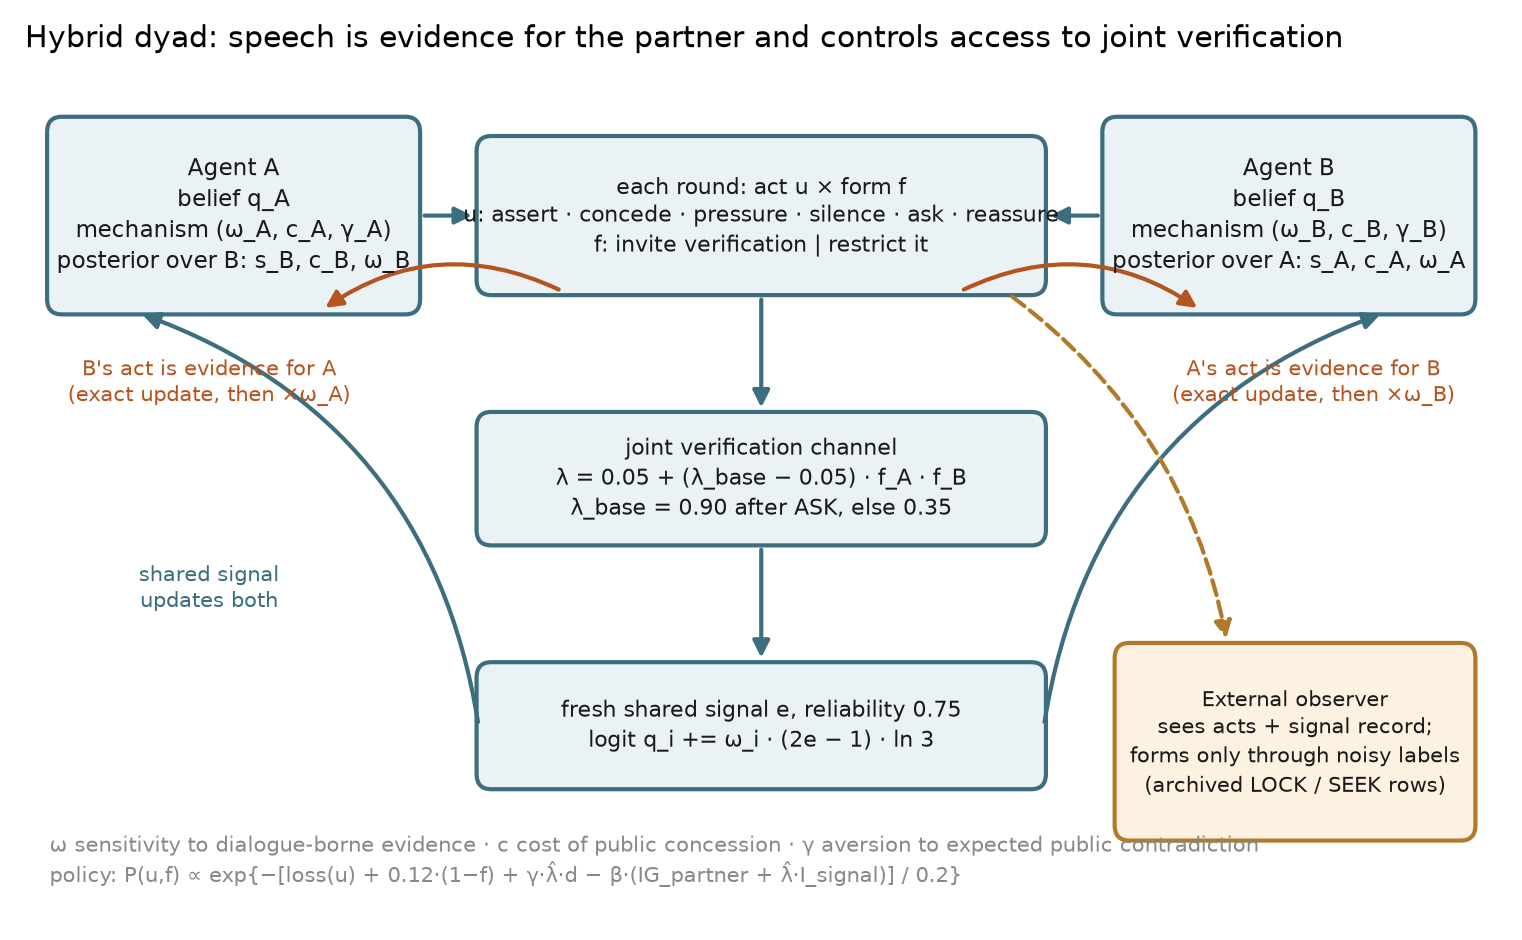
\includegraphics[width=0.9\textwidth]{../figures/H0_model_schematic.png}\end{center}
Both agents infer; each move is an \textbf{act} $u\in\{$ASSERT, CONCEDE, PRESSURE, SILENCE, ASK, REASSURE$\}$ $\times$ a \textbf{form} $f\in\{$invite, restrict$\}$. A fresh shared signal arrives with
\[
\lambda_t=0.05+(\lambda_{\mathrm{base}}-0.05)\,f_{A}f_{B},\quad \lambda_{\mathrm{base}}=0.35\ (0.90\text{ after ASK}),
\]
so one restricting form collapses the channel to its floor. Policy over act$\times$form:
\begin{align*}
G(u,f)&=\ell(u)+\delta(1-f)+\gamma\,\lambda(u,f)\,d_t\\
&\quad-\beta\big[\lambda(u,f)\,\Iw+\mathrm{IG}_{\text{partner}}(u)\big],\\
P(u,f)&\propto e^{-G(u,f)/\tau},
\end{align*}
$\delta=0.12$, $\beta=1.5$, $\tau=0.2$;
$d_t$ = probability that the next signal contradicts one's position. The partner's act is evidence through a level-0 model of the partner; every update is exact Bayes, then the $x$-marginal moves a fraction $\omega$ of the way (marginal shrink; the signal term $\Iw$ is a stated heuristic, off by $\le0.014$ nat at $\omega=0.2$).

\medskip
\textbf{External observer} (the ``annotator''): sees acts and the signal record, computes the exact posterior over the speaker's mechanism family; forms only through labels drawn from the LOCK / SEEK rows. Null channel: labels drawn from the \emph{act} instead of the form. Oracle: true forms. Ten validation checks pass; reproduces the M-bridge prototype act-for-act and the reciprocal dyad to $3\cdot10^{-12}$.
\end{block}

\begin{block}{6 \; Design: simulated dialogues per group for 80\,\% power (Welch, $\alpha=0.05$)}
{\small\begin{tabular}{@{}lrrr@{}}
\toprule
 & atten.\ vs cost & atten.\ vs access & cost vs access\\
\midrule
late non-concession & 200 & 35 & 25\\
private belief change & \textbf{17} & 25 & $>400$\\
restriction rate & $>400$ & \textbf{12} & \textbf{12}\\
listener $P(\omega_A{=}0.2)$ & \textbf{12} & 12 & $>400$\\
listener $P(c_A{=}1.6)$ & 25 & 50 & \textbf{12}\\
\bottomrule
\end{tabular}
\smallskip

Each mechanism has one cheap channel; none separates all three pairs.
}
\end{block}

\end{column}

%%%%%%%%%%%%%%%%%%%%%%%%%%%%%%%%%%%%%%%%%%%%%%%%%%%%%%%%% column 3
\begin{column}{0.315\textwidth}

\begin{block}{7 \; Three mechanisms, three channels (speaker A, honest partner, $n=1\,381$)}
\begin{center}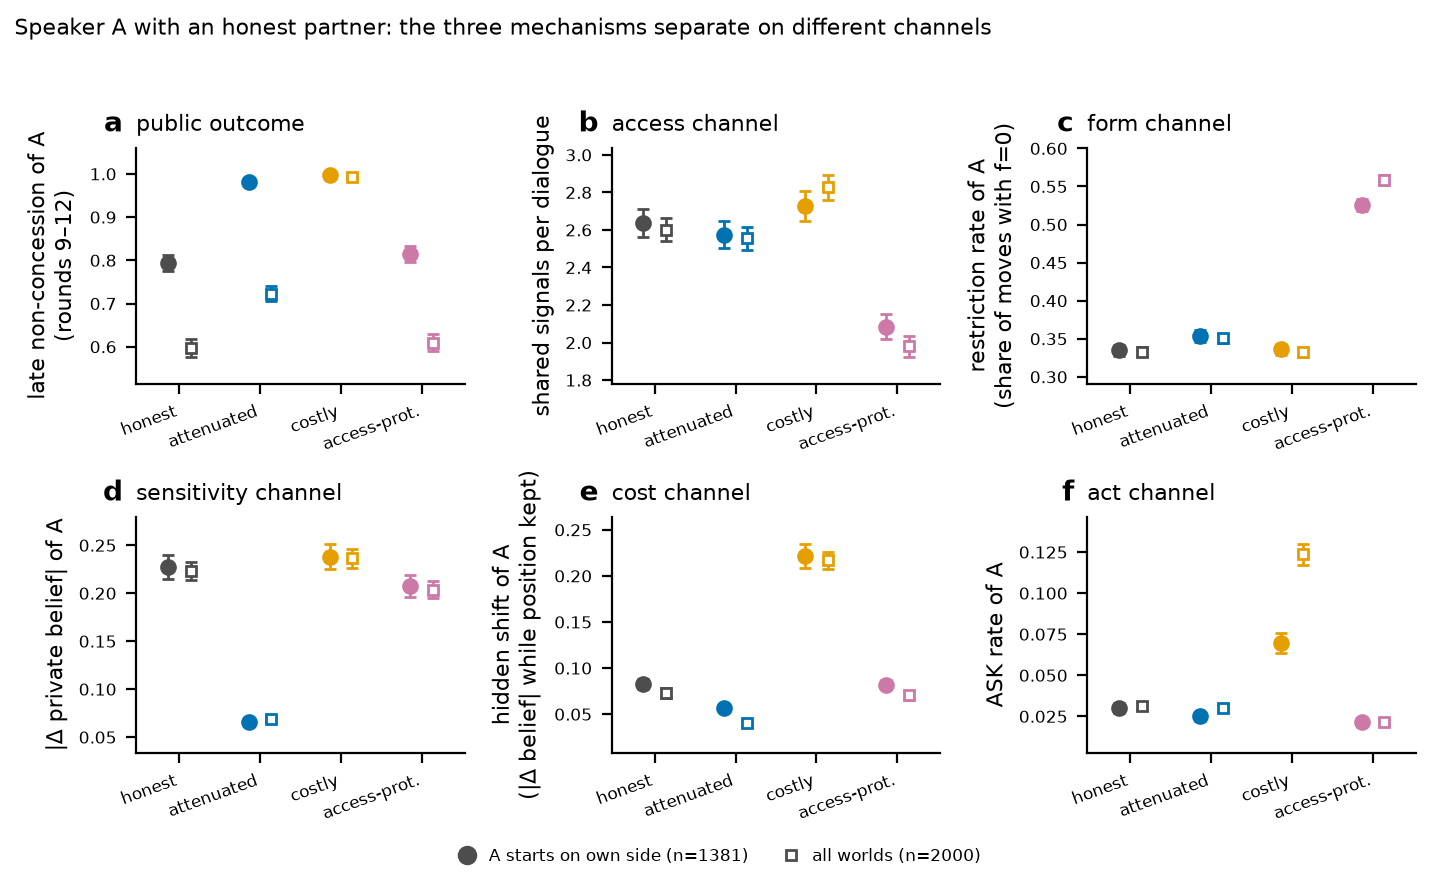
\includegraphics[width=\textwidth]{../figures/H1_channels.png}\end{center}
{\small\begin{tabular}{@{}lrrrr@{}}
\toprule
channel & honest & $\omega{=}0.2$ & $c{=}1.6$ & $\gamma{=}2$\\
\midrule
late non-concession & 0.79 & \textbf{0.98} & \textbf{1.00} & 0.81\\
$|\Delta$ private belief$|$ & 0.23 & \textbf{0.07} & 0.24 & 0.21\\
hidden shift (belief moved, position kept) & 0.08 & 0.06 & \textbf{0.22} & 0.08\\
shared signals per dialogue & 2.64 & 2.58 & 2.73 & \textbf{2.09}\\
restriction rate & 0.34 & 0.35 & 0.34 & \textbf{0.53}\\
\bottomrule
\end{tabular}}
\smallskip

Attenuated and costly speakers are publicly identical and privately opposite: one does not learn, the other learns and hides it. The access protector does not look stubborn and learns normally from what arrives --- it arranges for less to arrive. This is trajectory~B formalised.
\end{block}

\begin{block}{8 \; Each mechanism answers to its own lever}
\small\begin{itemize}\setlength{\itemsep}{1pt}
\item \textbf{Partner's REASSURE} (net of placebo) and \textbf{removing $c$} move only the costly speaker's late concession: $+0.155$ and $+0.275$.
\item \textbf{Removing $\gamma$} moves only the access protector: $+0.199$ shared signals, $-0.187$ late restriction.
\item \textbf{One strong shared observation} moves the attenuated speaker least: $+0.058$ vs $+0.09$--$0.12$.
\item \textbf{Forcing the partner to invite} helps the access protector least ($+0.13$ vs $+0.31$--$0.33$ signals); it restricts more in return.
\item \textbf{The listener's own posterior} flags the costly ($P(c_A{=}1.6)=0.45$) and the attenuated speaker ($P(\omega_A{=}0.2)=0.59$).
\end{itemize}
\end{block}

\begin{block}{9 \; What the Part I labels buy the observer}
{\small\begin{tabular}{@{}lrrrr@{}}
\toprule
P(true family) & acts+signals & +labels & +oracle & null\\
\midrule
attenuated & 0.612 & \textbf{0.672} & 0.678 & 0.612\\
costly & 0.690 & \textbf{0.765} & 0.785 & 0.690\\
access-protecting & 0.681 & \textbf{0.756} & 0.812 & 0.681\\
\bottomrule
\end{tabular}}
\smallskip

Form labels add $+0.06$ to $+0.08$ and transmit 53--61\,\% of the oracle's information about the next signal; labels that only re-encode the act add exactly zero; labels add $\le0.006$ nat to next-\emph{act} prediction. Labels are informative \emph{only because} the form has a stipulated consequence for what gets checked.

\end{block}

\begin{alertblock}{10 \; What is and is not claimed}
\small\begin{itemize}\setlength{\itemsep}{1pt}
\item All bridge results are \textbf{simulations of stipulated mechanisms}; no human data.
\item The form $\to$ access rule, and the transport of two confusion rows to synthetic dyads, are assumptions to be estimated in real dyads.
\item An independently written dyad with different design choices reproduces the access result; with $\omega$ on shared signals only its attenuated speaker looks honest: the sign of ``strong evidence'' tests depends on where attenuation is localised.
\item Part I: the engine loses to a direct prompt; the keyword baseline was tuned on the scored cases; no gate ablation.
\item Regime persistence adds nothing to next-act forecasting in the reciprocal dyad; no physiological cost is modelled.
\end{itemize}
\end{alertblock}

\begin{block}{11 \; What to measure next in real dyads}
\small Private belief before and after (separates uptake from expression, $\approx17$ dialogues per group in simulation); whether each move \textbf{invites or restricts} verification and how much verification actually occurs (separates access, $\approx12$); the partner's estimate of the speaker; evidence exposure under a randomised incentive. The decisive test for the annotation: does invite/restrict coding of real dyads predict subsequent verification and belief change beyond action counts?
\end{block}

\end{column}
\end{columns}
\vfill
\begin{columns}[t,totalwidth=0.965\paperwidth]\begin{column}{\textwidth}
{\small\color{meta} All bridge quantities are simulation constructs (2\,000 worlds per condition, paired 95\,\% Monte Carlo intervals); mechanisms are stipulated; no human data. Paper: Svet, M. (2026) \emph{Speech that Protects a Model: Typed Speech Evidence and Belief-Protecting Mechanisms in a Dialogue Dyad}, IWAI 2026. Code MIT, text and figures CC BY 4.0. Models built with AI research assistants; design decisions and interpretations are the author's.}
\end{column}\end{columns}
\end{frame}
\end{document}
